\chapter{Spectrum Sensing}

Due to limited availability of spectrum resource, there is a serious impact on 
the emerging mobile applications. Hence there is a need to efficiently utilize
the available radio spectrum. The problem right now is not the physical scarcity
of the radio spectrum rather the inefficient use of the spectrum. Solution to 
this is cognitive radio. The major problem in cognitive radio is to detect 
spectrum holes which can be utilized by secondary users for communication and
to enable secondary users to quit the 
frequency band as soon as the corresponding primary radio emerges. This
technique is called spectrum 
sensing. Spectrum sensing is the first step to implement cognitive radio system.

There are various methods for local spectrum sensing proposed by researchers.

The following section describes three important methods:
\begin{enumerate}
	\item Energy detection
	\item Matched filter detection 
	\item Cyclostationarity detection
\end{enumerate}

\section{Energy Detection}

Measuring the energy of a particular band is one of the simplest techniques to 
detect the presence of primary users in that band. It is one of the most widely
used technique to detect spectrum holes as it requires no a priori knowledge of 
the primary radio. Apart from this major advantage the technique is very cost 
efficient and less complex compared to other techniques. 
We calculate the energy of the received radio spectrum and this energy is 
compared with a predefined energy detection threshold to conclude whether 
primary user is present or absent in the frequency of interest. This technique 
is an optimal one when we have absolutely no knowledge of the user occupying the
channel in advance. The following block diagram describes energy detection 
technique:

\begin{figure}[h]
\centering
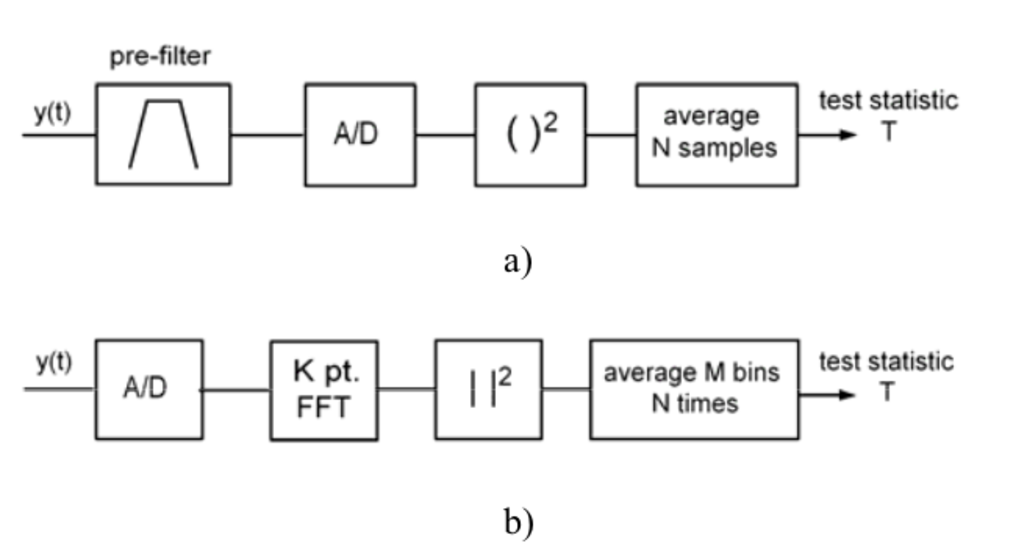
\includegraphics[width=0.8\textwidth]{../images/energyDetection}
\caption[Block diagram of Energy Detection implementatio]{Block diagram 
of Energy Detection implementation{\cite{cabric06}}.}
\label{energyDetection}
\end{figure}

As described in the energy detection block diagram, it is basically a hypothesis
testing problem with two possible hypothesis $H_0$ and $H_1$. Hypothesis $H_1$ concludes 
the presence of primary users in the band of interest and hypothesis $H_0$ 
concludes their absence. And energy detection technique is basically about 
distinguishing between these two hypotheses\cite{sarijari09}.


\begin{align}
  H_0: \qquad x(t) & = n(t);  \nonumber \\
  H_1: \qquad x(t) & = hs(t)+n(t);  \nonumber
\end{align}

$x(t)$ is signal received by secondary user and $s(t)$ is primary radio 
signal, $n(t)$ is additive white Gaussian noise (AWGN) and $h$ is the amplitude gain
of the channel. $s(t)$ and $n(t)$ are assumed to be independent of each other. 
Signal detection is performed using an energy detector and compute decision 
statistics $Y$ which corresponds to energy collected in observation time $T$ and 
bandwidth $W$ and comparing this statistics to a predetermined threshold
$\gamma$. In our project energy 
detection is implemented using average periodogram analysis which is covered in 
later part of this chapter.


\section{Matched filter detection}
Matched filter is a linear filter used to match a particular transit waveform 
with the reference signal. The output is maximum when the match happens. When 
there is a priori knowledge of primary radio, matched filter technique is 
applied. Matched filter operation is equivalent to correlation operation in 
which the incoming signal is convolved with a filter whose impulse response is 
mirror and shifted version of reference signal. This output is then compared 
with the threshold for primary user detection. It is mathematically defined as:

\begin{equation*}
Y[n] = \sum_{k=-\infty}^{\infty}x[k]h[n-k]
\end{equation*}

$x$ is the unknown signal and $h$ is the impulse response of matched filter which is 
matched to reference signal for maximizing SNR. 

\begin{figure}[h]
\centering
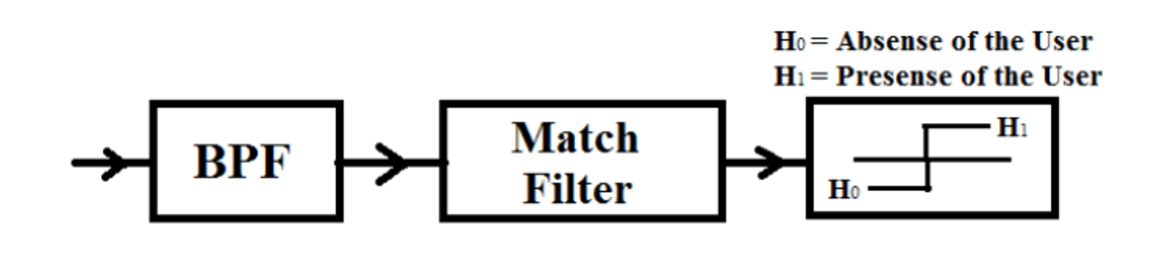
\includegraphics[width=0.8\textwidth]{../images/matchedFilter}
\caption[Matched Filter implementation]{Block diagram 
of Matched Filter implementation {\cite{kranthi13}}.}
\label{matchedFilter}
\end{figure}

There is a constraint on this technique. We need to have a prior information 
about the primary radio to perform matched filtering. However matched filter 
requires demodulation of primary signal which means it has information of 
primary radio both at the PHY layer and the MAC layer like operating frequency, 
modulation type, packet format bandwidth etc. But the cumbersome part is it has 
to achieve coherency with primary user by means of timing and carrier 
synchronization. This coherent detection is still achievable since primary 
signals have pilots, preambles etc to serve the purpose. 
The advantage of matched filter detection is when the information of the primary
user signal is known, it is optimal detection in stationary Gaussian noise. But 
the performance of matched filter detection depends on the accuracy of the 
information of primary radio. This technique also requires cognitive radio to 
have dedicated receiver for every type of primary user which in turn results in 
complex hardware and large power consumption\cite{mansi11}.

\section{Cyclostationarity detection}

This technique utilizes periodicity property of the received signal to detect 
the
presence of primary users. The property of Periodicity is generally exhibited by 
communication signals due to sinusoidal carriers, pulse train, hopping sequences
etc. Due to this underlying periodicity most of the communication signals can be
modeled as cyclostationary processes. This 
technique can detect a primary signal with a particular modulation type even in a
background of noise and other modulated signals.

Cyclostationary feature detection is robust to noise and is a better performer 
than energy based detection in low SNR regions. This technique also requires a 
priori knowledge of the primary signal. Also this technique is computationally 
highly complex and the sensing time is also quite long. Due the these reasons 
it is less commonly used than energy based detection.

Block diagram of cyclostationary detection is given in figure \ref{csd}
\cite{mansi11}.


\begin{figure}[h]
\centering
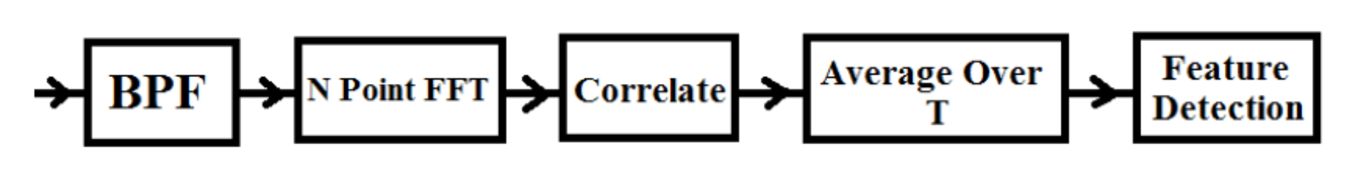
\includegraphics[width=0.8\textwidth]{../images/csd}
\caption[Cyclostationary Detection implementation]{Block diagram 
of Cyclostationary Detection implementation {\cite{mansi11}}.}
\label{csd}
\end{figure}
 

The detection is done by finding a unique cyclic frequency of the spectral 
correlation function of the received signal\cite{cabric04}. The spectral correlation 
function is the Fourier transform of the cyclic autocorrelation function. The 
spectral correlation function is defined as:
\begin{equation*}
        S(f,\alpha) = \int_{-\infty}^{\infty} R_{x}^{\alpha}(\tau)e^{-2 \pi f\tau}d\tau 
\end{equation*}
Where the cyclic autocorrelation function is defined by:
\begin{equation*}
    R_{x}^{\alpha} = E\{x(t+\tau)x^{*}(t-\tau)e^{-2 \pi \alpha t}\}
\end{equation*}
Here $x(t)$ is the signal received and $\alpha$ is the cyclic frequency. The spectral 
correlation function is also termed as cyclic spectrum.

We can also get the SCD function by considering a zero mean signal $x(t)$
whose time varying autocorrelation function $R_x(t,\tau)$ defined as
\cite{prithvi11}
\begin{equation*}
    R_{x}(t,\tau) = E\{x(t)x^{\ast}(t+\tau)\}
\end{equation*}
is periodic in time $t$ and can be represented as a Fourier series
\begin{equation*}
    R_{x}(t,\tau) = \sum_{\alpha}R_{x}^{\alpha} (\tau)e^{i2\pi\alpha t} 
\end{equation*}
for which the cyclic autocorrelation function is defined as
\begin{equation*}
    R_{x}^{\alpha}(\tau) = \lim_{T\rightarrow\infty} {\frac{1}{T}}
    \int_{\frac{T}{2}}^{\frac{T}{2}}R_{x}(t,\tau)e^{-i2\pi\alpha t}dT
\end{equation*}
Again the Fourier transform of $R_{x}^{\alpha}(\tau)$ is the SCD defined as
\begin{equation*}
    S_{x}^{\alpha}(\tau)=\int_{-\infty}^{\infty}R_{x}^{\alpha}
    (\tau)e^{-i2\pi f\tau}d\tau
\end{equation*}

This is a two-dimensional transform unlike power spectral density which is 
one-dimensional. For successful detection under cyclo-stationary based spectrum 
sensing, we need a priori knowledge of the cyclo-stationary features of the 
received signal only. However matched filtering is the optimal solution when we 
completely know about received signal in advance.
This technique doesn't work well when the underlying noise is stationary. More 
over channel fading destroys the property of cyclo stationarty of the received 
signal and is also susceptible to sampling clock offset. 


\section{Comparision of various spectrum detection techniques}


\begin{figure}[h]
\centering
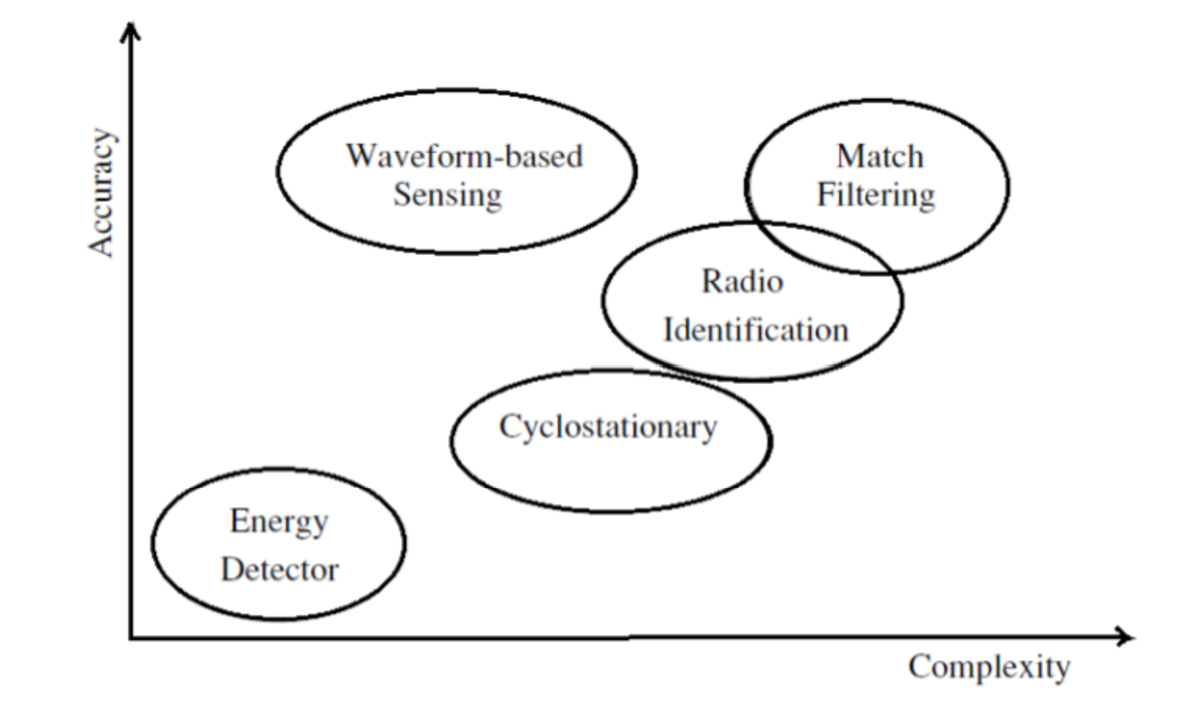
\includegraphics[width=0.8\textwidth]{../images/compareSensing}
\caption[Comparison of sensing methods]{Comparison of sensing methods {\cite{kranthi13}}}
\label{compareSensing}
\end{figure}
Figure \ref{compareSensing} compares various spectrum sensing techniques on
the basis of their 
accuracy and complexity. We can see that energy detection technique is the least
accurate and least complex of all where as matched filtering is most complex and
highly accurate. Other techniques lie in between with some having more accuracy 
and some less complex. There is no ideal detector that suits all occasions. Thus
decisions, compromises and tradeoffs must be made depending on primary radio 
type, transmission and propagation characteristics, characteristics of secondary
user receiver, and etc\cite{akyildiz06}.

\section{Implementaton of energy detection technique}
We have used energy detection technique for spectrum sensing in our project for 
the detection of primary users in the band of interest. Average periodigram 
analysis is a method to implement energy detection technique of spectrum 
sensing. This section describes average periodogram analysis.  Implementation of
wide band spectrum analyzer using this technique is also described in this 
section.

\subsection{Average periodogram analysis}
Average Periodogram analysis estimates the power spectrum of the received signal
and it is based on the Discrete Fourier Transform (DFT) of finite length 
segments of signal. In this technique signal is sectioned into finite length 
segments and periodogram of each segment is calculated which are also referred 
to as modified periodograms. Then an average of all these modified periodogram 
is calculated\cite{welch67}.

Let $X[n]; n = 0,1...L-1$ be the discrete time signal which is  divided into 
$M$ 
finite length segments of equal length, where $N$ is the length of each segment  
i.e. $ MN = L; X_{r}[n]; n = 0,1...N-1 $ is the $r$th segment and
$ W[n]; n = 0,1...N-1 $ is 
the window applied to each segment. The modified periodogram for the $r$th segment
 is,
\begin{equation*}
    I_{r}[k] = \frac{1}{NU} \left| V_{r}[k]\right|^2     \qquad k = 0,1...N-1 
\end{equation*}
where $V_{r}[k]$ is a N point DFT and $U$ is normalization factor i.e. , 
$V_{r}[k] = DFT\{W[n]*X[n]\}$
and $U = \frac{1}{N}(\sum_{n-0}^{N-1} (W[n])^2)$. The PSD of $X[n]$ sequence 
is then the time averaged periodogram estimate ,
\begin{equation*}
    I[k] = \frac{1}{M}\left|\sum_{r=0}^{M-1}X_{r}[k]\right|
\end{equation*}

\section{Wide band spectrum analyzer}

GNU radio packages provide a tool for wide band spectrum sensing called 
usrp\_spectrum\_sense.py. 
It is used as a basic code for wide band spectrum analyzer implementation. The
output of this 
code is the magnitude squared of the FFT. This means for each FFT bin[i] the output 
is $ Y[i] = re[X[i]]*re[X[i]] + im[X[i]]*im[X[i]]$. We can calculate the power by
taking square root of the output. We need $N$ time samples of $x(t)$ sampled at a 
sampling frequency of $F_{s}$ to use $N$ point complex FFT $X(\omega)$ analysis. An 
appropriate window function is to be selected to reduce spectral leakage and 
applied to these time samples. The output of the complex FFT will represent the 
frequency spectrum content as follows: The first value of the FFT output 
$(bin0 == X[0])$ is the passband centre frequency The first half of FFT 
spectrum ($X[1]$ to $X[N/2-1]$) contains the positive baseband frequencies,
which corresponds
to the passband spectrum from centre frequency to $+F_{s}/2$. The second half of the 
FFT ($X[N/2]$ to $X[N-1]$) contains the negative baseband frequencies, i.e. from 
$-F_{s}/2$ to centre frequency.



For our project purpose, we collected 1024 samples using a tuner centered at 
uplink frequency of our interest, say 900 MHz. 1024 is choosen as the number of 
FFT points because the number of FFT points has to be a power of 2 for the fast 
execution of the FFT algorithm. Default  sampling frequency is set as 1 MHz. 
The frequency resolution is therefore: 1 MHz / 1024 = 976.56 KHz. The 
decimation is defined as dsp rate divided by sample rate. The UHD driver 
requires the decimation value to be an even number. The dsp rate is the actual 
hardware-level sampling rate of the USRP kit. It is the rate at which the USRP 
device takes analog samples from the external world and converts them to digital
form. The dsp rate of the USRP is 100 MHz. Hence we chose sampling frequency to 
be 1 MHz which gives a decimation value of: 100 MHz / 1 MHz = 100.

A GSM band is of 200 KHz. So, in order to calculate the energy in a particular
frequency channel of interest, we need to find the average of all the bin values
which lie in the 200 KHz band centered at that frequency.